\newpage
\section{Аналитическая часть}

\subsection{Описание задачи}

Конвейеризация – это техника, в результате которой  задача или  команда разбивается  на некоторое число подзадач, которые  выполняются последовательно. Каждая  подкоманда   выполняется на своем логическом  устройстве.    Все     логические    устройства   (ступени)  соединяются последовательно таким образом, что выход  $i$-ой   ступени   связан   с   входом   $(i+1)$-ой   ступени,  все ступени  работают  одновременно.  Множество  ступеней называется    конвейером.    Выигрыш     во    времени достигается при  выполнении  нескольких задач  за  счет параллельной   работы   ступеней,  вовлекая  на  каждом такте новую задачу или команду \cite{Conveer}.

В конвейере различают $r$ последовательных этапов, так что когда $i$-я операция
проходит $s$-й этап, то $(i+k)$-я операция проходит $(s-k)$-й этап.

\begin{figure}[H]
    \center{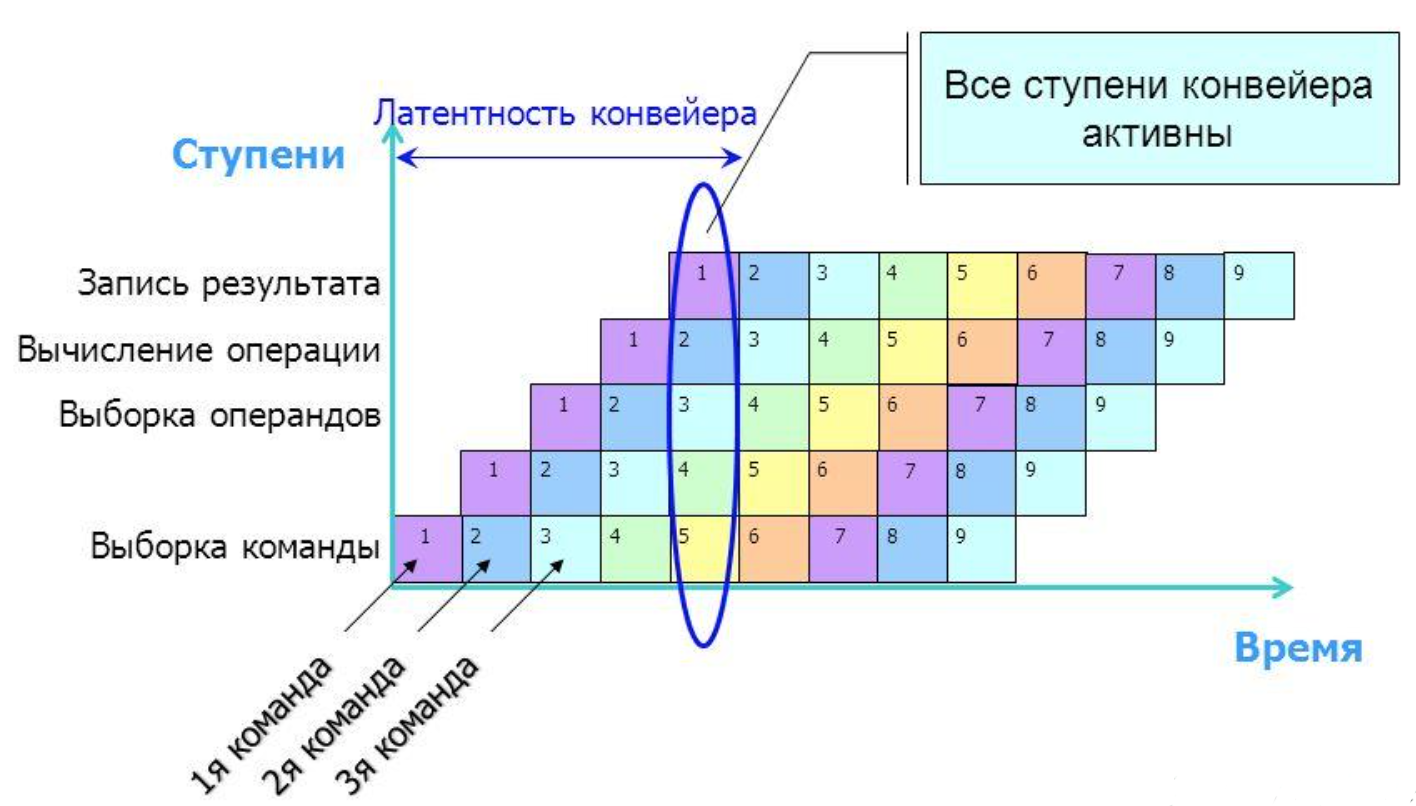
\includegraphics[scale=0.5]{conveer_img}}
    \caption{Работа конвейра}
    \label{img:conveer}
\end{figure}

\subsection{Выводы}

Таким образом, выигрыш во времени достигается при выполнении нескольких задач за
счет параллельной работы ступеней, вовлекая на каждом такте новую задачу или
команду. Однако работу конвейера тормозят зависимости  по данным и конфликты по ресурсам.
